% BGIN Block 15 — the IKP co-chair's four sessions (15–16 Oct 2026, Georgetown University Capitol Campus)
% 1-4 / 1-7 PQC Migration (Room B, 15 Oct 09:50–13:00) · 2-6 Privacy Enhanced Authentication, ZKP & Proof of
% Personhood (Room B, 16 Oct 11:30–13:00) · 2-9 AML Policy, Forensics & Analytics — Common Taxonomy (FASE/IKP,
% Room A, 16 Oct 15:40–17:10, with Chloe White).
% House style of the GDC26 / Block 15 PQC decks: dark title bar, grey lead box, "Takeaway" line, BGIN mark in the footer.
% Facts follow the Block 15 programme (bgin-global.org/events/20261015-block15), bgin-global/pqc-agility-competition
% (draft v0, main 86c780a), the Block 14 meeting reports, the proof-of-human convergence note (Aug 2026) and the
% IKP KB in ~/BGIN_IKP. Everything shown is unratified.
% Build: latexmk -pdf Block15_IKP_CoChair_Sessions.tex
\documentclass[aspectratio=169,10pt]{beamer}
\usepackage[utf8]{inputenc}
\usepackage[T1]{fontenc}
\usepackage{helvet}
\renewcommand{\familydefault}{\sfdefault}
\usepackage{booktabs}
\usepackage{array}
\usepackage{graphicx}
\usepackage{fontawesome5}
\usepackage{tikz}
\usetikzlibrary{arrows.meta,positioning,calc}
\usepackage{qrcode}
\usepackage{hyperref}

\usetheme{default}
\setbeamersize{text margin left=7mm,text margin right=7mm}
\setlength{\tabcolsep}{4pt}
\definecolor{bar}{RGB}{25,25,29}
\definecolor{ink}{RGB}{35,35,40}
\definecolor{soft}{RGB}{110,110,118}
\definecolor{boxbg}{RGB}{242,242,244}
\definecolor{lane}{RGB}{225,227,232}
\definecolor{pqc}{RGB}{247,147,26}
\definecolor{pop}{RGB}{92,74,140}
\definecolor{popbg}{RGB}{236,233,244}
\definecolor{aml}{RGB}{18,108,108}
\definecolor{amlbg}{RGB}{228,240,239}
\setbeamercolor{normal text}{fg=ink}
\setbeamercolor{structure}{fg=bar}
\setbeamercolor{frametitle}{bg=bar,fg=white}
\setbeamercolor{block body}{bg=boxbg,fg=ink}
\setbeamercolor{pop body}{bg=popbg,fg=ink}
\setbeamercolor{aml body}{bg=amlbg,fg=ink}
\setbeamertemplate{navigation symbols}{}
\setbeamertemplate{itemize item}{\color{bar}\faAngleRight}
\setbeamertemplate{itemize subitem}{\color{soft}\textendash}
\setbeamertemplate{enumerate item}{\colorbox{bar}{\color{white}\scriptsize\insertenumlabel}}
\setbeamerfont{frametitle}{series=\bfseries,size=\large}
\setbeamertemplate{frametitle}{%
  \vskip-2pt\begin{beamercolorbox}[wd=\paperwidth,ht=8mm,dp=2.5mm,leftskip=6mm]{frametitle}%
  \usebeamerfont{frametitle}\insertframetitle\hfill{\small\mdseries\insertframesubtitle}\hspace{6mm}\end{beamercolorbox}}
\setbeamertemplate{footline}{%
  \begin{beamercolorbox}[wd=\paperwidth,ht=5mm,dp=2mm,leftskip=6mm,rightskip=6mm]{normal text}%
  \tiny\color{soft}\raisebox{-1.2pt}{
\includegraphics[height=3.2mm]{bgin_mark.png}}\hspace{1.2mm}%
  BGIN Block 15 --- IKP Working Group sessions\hfill Washington, D.C. \textbar{} 15--16 Oct 2026 / \insertframenumber\end{beamercolorbox}}
\newcommand{\takeaway}[1]{\par\vspace{1.5mm}{\small\color{bar}\faLink~\textbf{Takeaway:} #1}}
\newcommand{\lead}[1]{\begin{beamercolorbox}[wd=\textwidth,sep=2.5mm]{block body}\small #1\end{beamercolorbox}\par\vspace{2mm}}
\newcommand{\poplead}[1]{\begin{beamercolorbox}[wd=\textwidth,sep=2.5mm]{pop body}\small #1\end{beamercolorbox}\par\vspace{2mm}}
\newcommand{\amllead}[1]{\begin{beamercolorbox}[wd=\textwidth,sep=2.5mm]{aml body}\small #1\end{beamercolorbox}\par\vspace{2mm}}
\newcommand{\pillar}[3]{\begin{minipage}[t]{#1}\colorbox{bar}{\parbox{\dimexpr\linewidth-2\fboxsep}{\color{white}\small\textbf{#2}}}\par\vspace{1mm}{\small #3}\end{minipage}}
\newcommand{\cpillar}[4]{\begin{minipage}[t]{#2}\colorbox{#1}{\parbox{\dimexpr\linewidth-2\fboxsep}{\color{white}\small\textbf{#3}}}\par\vspace{1mm}{\small #4}\end{minipage}}
% \sectiontitle{accent}{kicker}{title}{subtitle}
\newcommand{\sectiontitle}[4]{{\setbeamertemplate{footline}{}\begin{frame}[plain]
  \begin{tikzpicture}[remember picture,overlay]
    \fill[bar] (current page.north west) rectangle (current page.south east);
    \node[anchor=north east,inner sep=0] at ([xshift=-7mm,yshift=-5mm]current page.north east){
\includegraphics[height=1.9cm]{bgin_logo.png}};
    \node[anchor=south west,text=#1,font=\small\bfseries] at ([xshift=7mm,yshift=-2.9cm]current page.north west){#2};
    \node[anchor=south west,text=white,font=\Large\bfseries,text width=13cm,align=left] at ([xshift=7mm,yshift=-4.7cm]current page.north west){#3};
    \node[anchor=north west,text=white,font=\small,text width=13cm,align=left] at ([xshift=7mm,yshift=-5.0cm]current page.north west){#4};
  \end{tikzpicture}
\end{frame}}}
\hypersetup{colorlinks,urlcolor=bar,linkcolor=ink}
\newcommand{\nohyph}{\hyphenpenalty=10000 \exhyphenpenalty=10000 \relax}

\begin{document}

% ================================================================ 1 TITLE
{\setbeamertemplate{footline}{}
\begin{frame}[plain,t]
  \begin{tikzpicture}[remember picture,overlay]
    \fill[bar] (current page.north west) rectangle ([yshift=-3.1cm]current page.north east);
    \node[anchor=north east,inner sep=0] at ([xshift=-7mm,yshift=-5mm]current page.north east){
\includegraphics[height=1.9cm]{bgin_logo.png}};
    \node[anchor=west,text=white,font=\Large\bfseries] at ([xshift=7mm,yshift=-1.55cm]current page.north west){IKP at Block 15 --- Keys, Identity, Privacy};
    \node[anchor=west,text=white,font=\small,text width=11.2cm,align=left] at ([xshift=7mm,yshift=-2.45cm]current page.north west){PQC migration \textperiodcentered{} privacy-enhanced authentication, ZKP \& proof of personhood \textperiodcentered{} AML policy, forensics \& analytics};
    \node[anchor=west,font=\normalsize] at ([xshift=7mm,yshift=-4.5cm]current page.north west){Mitchell Travers \textperiodcentered{} Co-Chair, IKP Working Group \textperiodcentered{} BGIN};
    \node[anchor=north west,font=\small,text=soft,text width=13.2cm,align=left] at ([xshift=7mm,yshift=-4.9cm]current page.north west){BGIN Block \#15 \textbar{} Georgetown University Capitol Campus, Washington, D.C. \textbar{} 15--16 October 2026 \textbar{} hybrid};
    \node[anchor=west,font=\scriptsize,text=soft,text width=13cm,align=left] at ([xshift=7mm,yshift=-6.2cm]current page.north west){Four sessions chaired by the IKP co-chair: 1-4 and 1-7 (15 Oct, Room B) \textperiodcentered{} 2-6 (16 Oct, Room B) \textperiodcentered{} 2-9 with Chloe White, FASE (16 Oct, Room A) \textperiodcentered{} every draft shown is open for comment; nothing is ratified};
  \end{tikzpicture}
\end{frame}}

% ================================================================ 2 the track in one page
\begin{frame}{The IKP Track at Block 15 in One Page}
  \lead{Identity, key management and privacy: three threads, four chaired sessions, one keynote and one lunch that set them up. Two further joint sessions are chaired by Cyber Security with IKP contributing.}
  \begin{center}\scriptsize
  \begin{tabular}{@{}p{1.0cm}p{2.5cm}p{1.2cm}p{5.4cm}p{3.6cm}@{}}\toprule
    \textbf{Slot} & \textbf{When} & \textbf{Room} & \textbf{Session} & \textbf{Who}\\ \midrule
    1-2 & 15 Oct 09:20--09:50 & A & Keynote: \emph{Crypto Agility in the Quantum and AI Era} & Alex Pruden, Project Eleven\\
    \textbf{1-4} & 15 Oct 09:50--11:20 & B & \textbf{IKP: PQC Migration (1)} --- resource estimates into judging criteria & Kanta Matsuura, Tadahiko Itoh; chair M.\,Travers\\
    \textbf{1-7} & 15 Oct 11:30--13:00 & B & \textbf{IKP: PQC Migration (2)} --- agility as governance, the NIST path, the W2 decisions & Kanta Matsuura, Tadahiko Itoh; chair M.\,Travers\\
    2-4 & 16 Oct 09:50--11:20 & B & Cyber + IKP: Security AI Agent --- information sharing \& vulnerability handling & chair J.\,Bringer\\
    \textbf{2-6} & 16 Oct 11:30--13:00 & B & \textbf{IKP: Privacy Enhanced Authentication, ZKP \& Proof of Personhood} & contributors; World as main discussant; chair M.\,Travers\\
    2-L & 16 Oct 13:00--14:00 & B & Industry lunch: World --- proof of personhood in practice & World\\
    2-8 & 16 Oct 14:00--14:45 & B & Cyber + IKP: Offline Key Management & chair J.\,Bringer\\
    \textbf{2-9} & 16 Oct 15:40--17:10 & A & \textbf{AML Policy, Forensics \& Analytics --- Common Taxonomy (FASE/IKP)} & chairs M.\,Travers, Chloe White\\ \bottomrule
  \end{tabular}
  \end{center}
  \takeaway{Each chaired session leaves with a record: a decision log for the competition, room comments into the personhood paper, and a publication path for the forensics-and-analytics document.}
\end{frame}

% ================================================================ 3 one group, three threads
\begin{frame}{One Working Group, Three Threads --- What Connects Them}
  \cpillar{pqc}{0.31\textwidth}{Keys over time}{PQC migration asks how a key stays trustworthy for decades on a public ledger: which keys are already exposed, how a stack switches schemes, and how a ``PQC-ready'' claim is measured rather than asserted.}\hfill
  \cpillar{pop}{0.31\textwidth}{Identity without disclosure}{Privacy-enhanced authentication asks how a counterparty proves it is a unique human, or an agent acting for one, while disclosing nothing else --- and what each proof actually establishes.}\hfill
  \cpillar{aml}{0.31\textwidth}{Inference and its limits}{Forensics and analytics ask what can be inferred from a public ledger, by whom, to what standard of evidence, and under what safeguards --- in a vocabulary two industries can share.}
  \par\vspace{2.5mm}
  {\small All three decide the same two things: \textbf{what a proof proves}, and \textbf{who is allowed to know}. A personhood credential that is unlinkable by design and a sanctions-screening duty that presumes identifiability meet in the same working group --- on purpose.}
  \takeaway{IKP's job this Block is to write the criteria, the taxonomy and the lexicon so the three answers are compatible --- not to pick a primitive, a provider, or a tool.}
\end{frame}

% ================================================================ 4 since Block 14
\begin{frame}{From Tokyo to Washington --- What Moved Since Block 14}
  \begin{columns}[T]
    \begin{column}{0.48\textwidth}
      {\small\textbf{Block 14 (Tokyo, March 2026) left on record}}
      \begin{itemize}\small
        \item Meeting reports: \emph{Crypto Agility and PQC Migration}; \emph{Privacy Enhanced Authentication and Key Management}; \emph{Proof of Personhood}; \emph{Forensics \& Analysis --- Common Lexicon of Harmful Activities}; \emph{Accountable Wallet}
        \item The three-graph personhood model and the dual-agent separation, with Block 15 named for public comment
        \item The common-lexicon mapping exercise, to start immediately
      \end{itemize}
    \end{column}
    \begin{column}{0.48\textwidth}
      {\small\textbf{On record since (public)}}
      \begin{itemize}\small
        \item GDC26 Geneva breakout (3 Sep): PQC migration on DLTs; Chatham House report
        \item Public coordination repository for the PQC Migration Prize: outcomes, governance, 22-metric register, scheme register, harness, roadmap W1--W6 --- all draft v0
        \item IKP research pathway on ZKP and private biometric authentication (July); topic-focused open IKP meetings on the personhood taxonomy; the proof-of-human convergence note (Aug)
        \item \emph{Distinguishing blockchain forensics from analytics} in public comment
      \end{itemize}
    \end{column}
  \end{columns}
  \takeaway{Every thread arrives at Block 15 with a public draft someone can argue with. The sessions are for the arguing.}
\end{frame}

% ================================================================ SECTION PQC
\sectiontitle{pqc}{Sessions 1-4 and 1-7 \textperiodcentered{} 15 October \textperiodcentered{} Room B \textperiodcentered{} 09:50--13:00}{PQC Migration: Resource Estimates into Criteria; Agility as Governance}{Workshop W2 of the PQC Migration Prize series. Session 1 turns the resource-estimate numbers into scored lines of a rubric. Session 2 writes the agility and governance rows, hears the NIST signature migration path, and takes the decisions. Speakers: Kanta Matsuura, Tadahiko Itoh.}

% ================================================================ 6 not another primitive
\begin{frame}{The Job Is Not to Pick Another Primitive}
  \lead{First PQC standards are in place (ML-KEM, ML-DSA, SLH-DSA; FN-DSA in draft; SP 800-208 stateful hash-based). Japan's PQC Migration Prize is hosted by METI/NEDO; BGIN coordinates internationally and runs the neutral evaluation testbed. It is not a BGIN contest, not a new-algorithm contest, and not chain endorsement.}
  {\small What still has no agreed playbook for public ledgers, wallets, and credentials:}
  \begin{itemize}\small
    \item How to stage a hybrid and then a cutover when every node must agree on validity rules.
    \item How to keep verifying old signatures for as long as funds and archives remain live.
    \item How to rotate keys and addresses without stranding dormant accounts.
    \item How to tell a genuine PQ-ready stack from a screenshot.
  \end{itemize}
  \takeaway{Treat PQC as a multi-year systems and governance program, not a weekend library swap. GDC26 named the gaps; Block 15 writes the criteria.}
\end{frame}

% ================================================================ 7 the numbers
\begin{frame}{Session 1-4 --- The Numbers on the Table}
  \lead{Migration urgency is a function of resource estimates. This room holds the estimate and the architecture in one place; policy rooms usually hear them from different speakers.}
  \begin{center}\small
  \begin{tabular}{@{}p{4.6cm}p{9.2cm}@{}}\toprule
    \textbf{Source} & \textbf{What it says}\\ \midrule
    Google Quantum AI et al., \emph{PRX Quantum} 7, 031001 (Aug 2026) & secp256k1 ECDLP at about 1{,}200 logical qubits and 90M Toffoli gates, or 1{,}450 / 70M; attacks sorted \textbf{on-spend / at-rest / on-setup}; mitigations ranked by on-chain consequence\\
    ECDSA.fail community benchmark & The continuing open resource-estimation benchmark: solvers and agents under public notes, re-run by a validator, promoted by measured improvement\\
    Project Eleven, \emph{Key recovery from state reuse} (Sep 2026) & The stateful hash-based failure is demonstrated, not theoretical: signing twice from one LMS / XMSS state exposes the key\\ \bottomrule
  \end{tabular}
  \end{center}
  \takeaway{The estimates set the clock. No calendar marketing of a single Q-day --- threat narratives are scenarios, and the register scores which keys are already public.}
\end{frame}

% ================================================================ 8 taxonomy
\begin{frame}{On-Spend, At-Rest, On-Setup --- Timing Is Not One Number}
  \pillar{0.31\textwidth}{On-spend}{The public key is revealed only when funds move. The race is between the legitimate owner and an attacker who sees the broadcast --- a fast-clock CRQC during confirmation, not an unbounded offline grind.}\hfill
  \pillar{0.31\textwidth}{At-rest}{The public key is already on-chain. Any CRQC, at any later date, can grind offline against the stored verification key and forge a spend.}\hfill
  \pillar{0.31\textwidth}{On-setup}{A universal classical exploit manufactured once by a one-off quantum computation, before any attack --- the case that breaks the ``we will see it coming'' assumption.}
  \par\vspace{2mm}
  {\small Address design, key reuse, and wallet defaults therefore change the threat model. Metric open question 6 asks, for each of the 22 metrics, which of the three classes it defends against. The same split returns in the Offline Key Management session (2-8): cold storage is at-rest by definition.}
  \takeaway{Resource estimates only become policy-useful when they are tied to which keys are already public.}
\end{frame}

% ================================================================ 9 estimate -> criterion
\begin{frame}{How an Estimate Becomes a Criterion}
  \lead{The register scores substantiation, not fear. Three rows carry the resource-estimate work; the rest are performance and agility.}
  \begin{itemize}\small
    \item \textbf{M-19 Security review score} --- checklist: assumptions, parameter set, side channels, stateful-key handling; seeds from the PQC Audit Index, to be adopted at W2.
    \item \textbf{M-22 PQC-readiness claim substantiation} --- checklist against the \emph{``PQC-ready chain'' definition}, the December (W4) deliverable; scores a stack against a published definition rather than a claim.
    \item \textbf{M-20 Governance fit} --- transition-period design, dormant / vulnerable asset treatment, the owner-versus-attacker race: a structured narrative, discussion input, not a policy decree.
    \item \textbf{Gate G1} --- the primitive is NIST-standardized or NIST-selected, or a committee-ruled hybrid / stateful hash-based scheme. No new primitives, ever.
  \end{itemize}
  \takeaway{An estimate enters the rubric as a declared assumption with error bars, scored under M-19 and M-22 --- never as a date.}
\end{frame}

% ================================================================ 10 three lanes
\begin{frame}{Three Lanes and What Gets Evaluated}
  \begin{center}
  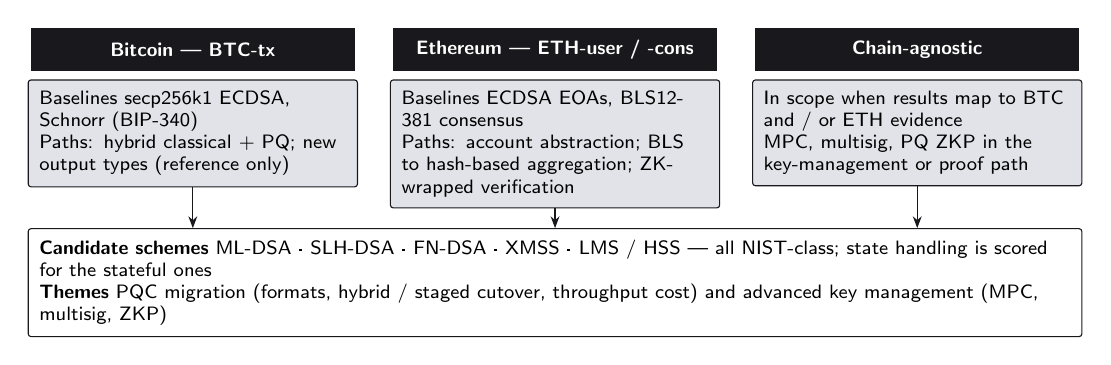
\begin{tikzpicture}[font=\scriptsize, box/.style={draw=bar,fill=lane,rounded corners=1pt,text width=3.9cm,align=left,inner sep=4pt}, hd/.style={fill=bar,text=white,font=\scriptsize\bfseries,text width=3.9cm,align=center,inner sep=3pt,minimum height=5.5mm}]
    \node[hd] (h1) at (0,0) {Bitcoin --- BTC-tx};
    \node[hd] (h2) at (4.6,0) {Ethereum --- ETH-user / -cons};
    \node[hd] (h3) at (9.2,0) {Chain-agnostic};
    \node[box,below=1mm of h1] (b1) {Baselines secp256k1 ECDSA, Schnorr (BIP-340)\\ Paths: hybrid classical + PQ; new output types (reference only)};
    \node[box,below=1mm of h2] (b2) {Baselines ECDSA EOAs, BLS12-381 consensus\\ Paths: account abstraction; BLS to hash-based aggregation; ZK-wrapped verification};
    \node[box,below=1mm of h3] (b3) {In scope when results map to BTC and / or ETH evidence\\ MPC, multisig, PQ ZKP in the key-management or proof path};
    \node[draw=bar,fill=white,rounded corners=1pt,text width=13.1cm,inner sep=4pt,align=left,below=2.5mm of b2.south,anchor=north] (ev) {\textbf{Candidate schemes} ML-DSA \textperiodcentered{} SLH-DSA \textperiodcentered{} FN-DSA \textperiodcentered{} XMSS \textperiodcentered{} LMS / HSS --- all NIST-class; state handling is scored for the stateful ones\\ \textbf{Themes} PQC migration (formats, hybrid / staged cutover, throughput cost) and advanced key management (MPC, multisig, ZKP)};
    \foreach \b in {b1,b2,b3} \draw[-{Stealth[length=1.5mm]},bar] (\b.south) -- (\b.south |- ev.north);
  \end{tikzpicture}
  \end{center}
  {\small Comparative scoring is anchored on Bitcoin and Ethereum. Every performance number is a ratio against the classical baseline on the same node, reproduced on $k$ nodes in at least two regions (gate G3).}
  \takeaway{Japan funds the prize. BGIN turns shared evidence into standards-ready artifacts. NIST remains the reference for which primitives are in scope.}
\end{frame}

% ================================================================ 11 agility
\begin{frame}{Session 1-7 --- Agility Is Harder Than Readiness}
  \lead{Evidence on the \textbf{mechanism of switching} --- hybrid and staged migration, scheme substitution cost, rollback, policy flexibility --- because the next migration is already certain and the primitive list will move again.}
  \begin{center}\scriptsize
  \begin{tabular}{@{}p{1.2cm}p{3.6cm}p{3.2cm}p{5.6cm}@{}}\toprule
    \textbf{Metric} & \textbf{What} & \textbf{Unit} & \textbf{How measured}\\ \midrule
    M-14 & Agility switch cost & time + coordination steps & scenario: swap scheme A to B under the proposed mechanism --- the core agility metric\\
    M-13 & Rollback cost & time + coordination steps & scenario: revert a staged migration\\
    M-12 & Migration throughput & keys / accounts per unit time & scenario; documents the user vs node-operator burden split\\
    M-21 & Legacy verification continuity & pass / fail + node cost & pre-migration signatures still verify after cutover\\
    M-20 & Governance fit & structured narrative & transition design, dormant assets, the owner-versus-attacker race --- recorded, not ruled\\ \bottomrule
  \end{tabular}
  \end{center}
  \takeaway{Agility written as a governance property is what lets the same rubric travel: competition $\rightarrow$ BGIN Standard $\rightarrow$ ISO/TC 307 $\rightarrow$ Japan's crypto-asset security criteria.}
\end{frame}

% ================================================================ 12 NIST path
\begin{frame}{The NIST Signature Migration Path --- What the Register Leans On}
  \lead{NIST is the algorithm and parameter authority for everything in scope; it is not a competition lane. Measurement-methodology cooperation is sought where appropriate, and NIST participation is invited in this session.}
  \begin{itemize}\small
    \item \textbf{FIPS 204 ML-DSA}, \textbf{FIPS 205 SLH-DSA} --- standardized; scheme rows S-01 and S-02.
    \item \textbf{FIPS 206 FN-DSA (Falcon)} --- draft; S-03 is confirmed at the scope ruling.
    \item \textbf{SP 800-208} XMSS and LMS / HSS --- stateful hash-based; S-04 and S-05 with state handling scored. Non-SP-800-208 parameterizations (hash-based aggregation with ZK-friendly hashes) need an explicit ruling.
    \item \textbf{ACVP / CAVP} wording is the correctness gate for calibration tracks.
    \item Hybrid / composite signatures follow the \textbf{IETF LAMPS} direction (C-01); the on-ramp signature candidates are \textbf{out of scope by gate G1}.
  \end{itemize}
  \takeaway{The register tracks NIST's list; it never extends it. When the list moves, the agility metrics are what say whether a stack can follow.}
\end{frame}

% ================================================================ 13 decisions
\begin{frame}{What Block 15 Decides --- the W2 Outputs}
  \begin{center}\scriptsize
  \begin{tabular}{@{}p{5.0cm}p{4.8cm}p{4.0cm}@{}}\toprule
    \textbf{Decision} & \textbf{Method} & \textbf{Lands as}\\ \midrule
    Committee seated (Phase A); chairs elected; second convener named & nominations + COI forms; formal vote & COMMITTEE.md roster\\
    OUTCOMES O1--O6 ratified (if not at W1) & formal vote, quorum of half & decisions/ record\\
    Metric register v0 $\rightarrow$ v1; directions per metric & rough consensus on the PR & evaluation/METRICS.md\\
    Scheme-scope rulings: C-01 hybrid, C-02 quantum-resistant output type as reference, S-04 non-SP-800-208 parameters, C-03 / C-04 / C-05 & formal vote per ruling & decisions/ records\\
    Open-benchmark model for calibration tracks & vote on decision 0001; recusals recorded & decisions/0001 accepted\\
    Open questions 1--6 assigned owners & conveners call it & workshop W2 record\\ \bottomrule
  \end{tabular}
  \end{center}
  \takeaway{Discuss on Discourse, record by pull request, rule by decision record. Every vote and every scope ruling gets an ADR. Nothing is final until the committee ratifies it and the host publishes the call.}
\end{frame}

% ================================================================ 14 open questions
\begin{frame}{PQC --- The Open Questions That Need Owners Today}
  \begin{enumerate}\small
    \item Is the headline quantity \textbf{total overhead} or \textbf{migration speed}? The rubric decides the weights.
    \item Who must upgrade first --- \textbf{node operators or users} --- and how does M-12 reflect the burden split?
    \item How to score the \textbf{owner-versus-attacker race} during a migration window (M-20)?
    \item Which \textbf{reference CPU class} and \textbf{reference tx mix / block} anchor M-03 to M-09? Decision record 0002 territory, with $k$ and the tolerance band.
    \item Are \textbf{consensus-layer} (ETH-cons) and \textbf{user-level} (BTC-tx, ETH-user) evidence scored on one rubric or two?
    \item For each metric, which attack class --- \textbf{on-spend, at-rest, on-setup} --- does it defend against?
  \end{enumerate}
  \par\vspace{1mm}
  {\small Also for the room: what the \emph{``PQC-ready chain'' definition} has to contain for M-22 to be scorable by December; and whether the ECDSA.fail public-note discipline (model and harness named, re-run by a validator) is the admission rule for agent-produced numbers.}
\end{frame}

% ================================================================ 15 timeline
\begin{frame}{PQC --- From This Room to the 2028 Award}
  \begin{center}
  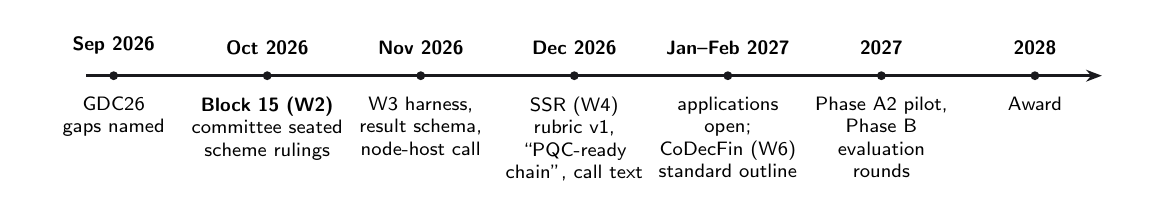
\begin{tikzpicture}[font=\scriptsize]
    \draw[line width=1pt,bar,-{Stealth[length=2mm]}] (0,0) -- (12.9,0);
    \foreach \x/\lab/\txt in {
      0.35/Sep 2026/{GDC26\\ gaps named},
      2.3/Oct 2026/{\textbf{Block 15 (W2)}\\ committee seated\\ scheme rulings},
      4.25/Nov 2026/{W3 harness,\\ result schema,\\ node-host call},
      6.2/Dec 2026/{SSR (W4)\\ rubric v1, ``PQC-ready\\ chain'', call text},
      8.15/Jan--Feb 2027/{applications open;\\ CoDecFin (W6)\\ standard outline},
      10.1/2027/{Phase A2 pilot,\\ Phase B evaluation\\ rounds},
      12.05/2028/{Award}}
      {\fill[bar] (\x,0) circle (1.6pt);
       \node[above=1.5mm,align=center,font=\scriptsize\bfseries] at (\x,0) {\lab};
       \node[below=1.5mm,align=center,text width=1.95cm] at (\x,0) {\txt};}
  \end{tikzpicture}
  \end{center}
  \par\vspace{1mm}
  \begin{center}\small
    Competition / evaluation $\rightarrow$ BGIN Standard $\rightarrow$ ISO/TC 307 $\rightarrow$ Japan's crypto-asset security criteria
  \end{center}
  {\scriptsize\color{soft} Dates are indicative until the host confirms the call. SSR 2026 PQC-for-blockchains workshop: Sun 13 Dec, Baltimore; peer-reviewed papers there are intended to be reflected in the competition specification.}
  \takeaway{This morning can still change what the call asks teams to prove. SSR on 13 December is the next drafting stop.}
\end{frame}

% ================================================================ SECTION PoP
\sectiontitle{pop}{Session 2-6 \textperiodcentered{} 16 October \textperiodcentered{} Room B \textperiodcentered{} 11:30--13:00, then lunch with World 13:00--14:00}{Privacy Enhanced Authentication, ZKP \& Proof of Personhood}{Authentication that proves the claim without disclosing the person. Builds on the two Block 14 reports and the open IKP meetings since: a high-level view of privacy-enhanced authentication, the taxonomy and the distinctions it has to keep (World as main discussant), verifiable trust agents acting for a person, and where zero-knowledge proofs do the work. Twenty minutes for contributors, then open discussion into the IKP proof-of-personhood paper.}

% ================================================================ 17 why now
\begin{frame}{Why Now --- Agentic AI Raises the Cost of Not Knowing}
  \poplead{When an AI system rather than a person can hold a wallet, pay, post and transact, every counterparty has to ask a question that used to be free: \textbf{is there a human here, and on whose authority is this agent acting?} The answer must not cost the human their privacy.}
  \begin{columns}[T]
    \begin{column}{0.48\textwidth}
      {\small\textbf{Block 14 left two reports}}
      \begin{itemize}\small
        \item \emph{Privacy Enhanced Authentication and Key Management}: one system holds the keys, another composes the transactions; AI as a separate process from the key holder, with scoped, revocable access
        \item \emph{Proof of Personhood}: the three-graph model, the dual-agent separation, the human stack, and the ISO TC 307 Technical Report path --- Block 15 named for public comment
      \end{itemize}
    \end{column}
    \begin{column}{0.48\textwidth}
      {\small\textbf{Since then}}
      \begin{itemize}\small
        \item IKP research pathway on ZK proofs for biometric authentication (July); open, topic-focused IKP meetings on the taxonomy
        \item A working note mapping three converging efforts: World's Proof of Human framework, the ToIP DTG credential and proof-of-liveness work, this paper
        \item Client-side ZK proving on everyday phones became real (ProveKit)
      \end{itemize}
    \end{column}
  \end{columns}
  \takeaway{The question is no longer whether personhood can be proven privately, but what a given proof proves, and to whom.}
\end{frame}

% ================================================================ 18 prove the claim
\begin{frame}{Prove the Claim, Not the Identity}
  \cpillar{pop}{0.31\textwidth}{What each proof proves}{Proof of \emph{a} human (uniqueness) is not proof of \emph{a specific} human (identity). A relying party should be told which one it is getting, at what strength, against which adversary --- and what the proof explicitly does not establish.}\hfill
  \cpillar{pop}{0.31\textwidth}{Where the biometric lives}{On the device, signed by the capture hardware and held by the person; uniqueness checked without an identity lookup (sMPC in World's design); government ID matched locally if at all. The architecture decides the harm if it fails.}\hfill
  \cpillar{pop}{0.31\textwidth}{Revocation of what cannot rotate}{A key can be rotated. An iris cannot. Revocation for a credential bound to a biometric means revoking the \emph{binding} and the \emph{enrolment}, not the person --- and saying so in the taxonomy.}
  \par\vspace{2.5mm}
  {\small Minimal disclosure and unlinkability are the two privacy properties every pattern here is scored on. Verifiability is not truth: a proof can be perfectly verifiable and still establish less than the relying party assumes.}
  \takeaway{A taxonomy that cannot say which of these a scheme delivers cannot be used to certify one.}
\end{frame}

% ================================================================ 19 the layers
\begin{frame}{Three Efforts, One Stack --- the Convergence Map}
  \poplead{Three efforts converged on the same structure independently. The friction is almost entirely at the seams between layers, which is where a working group earns its keep.}
  \begin{center}\scriptsize
  \begin{tabular}{@{}p{3.3cm}p{5.6cm}p{4.9cm}@{}}\toprule
    \textbf{Layer} & \textbf{Question it answers} & \textbf{Who is working here}\\ \midrule
    Assurance semantics & What class of claim, at what strength, on what evidence; how it maps to NIST xAL and ISO 29115 & World \emph{Proof of Human} framework (v0.13, Aug 2026: ten categories, four dimensions)\\
    Predicate semantics & What a proof establishes, what it does \emph{not}, what it discloses, to whom, against which adversary, for how long & ToIP DTG ZKP Task Force, proof-of-liveness requirements v0.4\\
    Mechanism & Which credential, protocol and proof construction carries the claim & DTG Core Credentials WD01; First Person Network\\
    Formal security & What the claim provably guarantees against a defined adversary & \emph{A Cryptographic Framework for Proof of Personhood} (ePrint 2026/333)\\
    Governance \& policy & Who may assert this, in what domain, under what regulatory consequence & \textbf{BGIN IKP}; trust registries; ISO TC 307\\ \bottomrule
  \end{tabular}
  \end{center}
  {\scriptsize\color{soft} Disclosure: the chair also co-chairs the ToIP DTG ZKP Task Force; observations on that work are personal and drawn from public materials.}
  \takeaway{Published standalone, a new taxonomy is a fourth competing vocabulary. Published as a layer bound to the predicates beneath it, it is what makes the others interoperable.}
\end{frame}

% ================================================================ 20 five distinctions
\begin{frame}{Five Distinctions the Taxonomy Has to Keep}
  \begin{center}\small
  \begin{tabular}{@{}p{3.0cm}p{10.8cm}@{}}\toprule
    \textbf{Distinction} & \textbf{Why it is load-bearing}\\ \midrule
    Humanity $\neq$ uniqueness & Two different claims, routinely collapsed into one credential. Liveness plus presence plus absence-of-automation is not the same as ``one person, once, in this domain''.\\
    Linkability scope & Adopt the architecture (pairwise, domain-scoped, global), then parameterise the dimension. A uniqueness assertion that survives across domains is a correlation key.\\
    Strength expression & The headline gap: how assurance is \emph{stated} rather than asserted --- ordinal scale, per-category scale, or a profile-defined vector a relying party can actually consume.\\
    Continuity & Continuity with enrolment is a property of the carrier and its controls, not of the primitive. Enrolment poisoning is its adversary.\\
    Agent authority & An agent acting for a human: the field list exists in the credential work; it needs completing with scope, delegation and revocation.\\ \bottomrule
  \end{tabular}
  \end{center}
  \takeaway{World is the main discussant here because its framework is strongest on strength expression and on separating humanity from uniqueness --- the two places the existing standards are thinnest.}
\end{frame}

% ================================================================ 21 three graphs + dual agent
\begin{frame}{The Block 14 Model --- Three Graphs, Two Agents}
  \begin{center}
  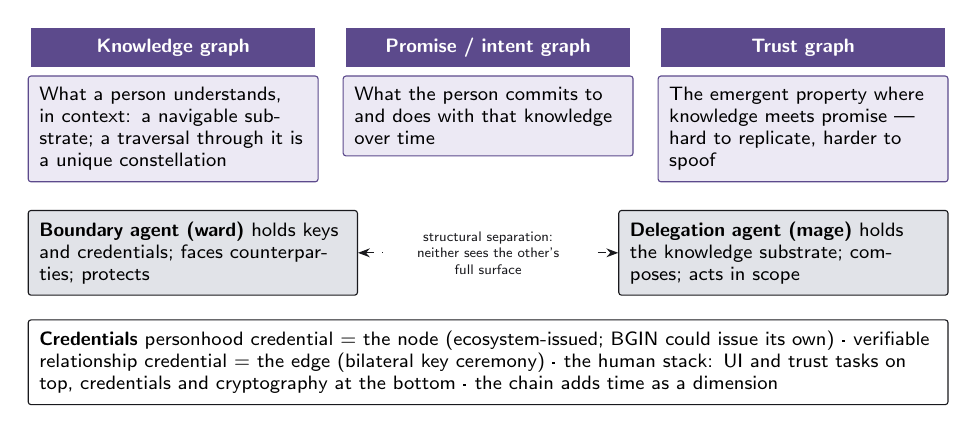
\begin{tikzpicture}[font=\scriptsize, g/.style={draw=pop,fill=popbg,rounded corners=1pt,text width=3.4cm,align=left,inner sep=4pt}, hd/.style={fill=pop,text=white,font=\scriptsize\bfseries,text width=3.4cm,align=center,inner sep=3pt,minimum height=5mm}, a/.style={draw=bar,fill=lane,rounded corners=1pt,text width=3.9cm,align=left,inner sep=4pt}]
    \node[hd] (h1) at (0,0) {Knowledge graph};
    \node[hd] (h2) at (4.0,0) {Promise / intent graph};
    \node[hd] (h3) at (8.0,0) {Trust graph};
    \node[g,below=1mm of h1] (g1) {What a person understands, in context: a navigable substrate; a traversal through it is a unique constellation};
    \node[g,below=1mm of h2] (g2) {What the person commits to and does with that knowledge over time};
    \node[g,below=1mm of h3] (g3) {The emergent property where knowledge meets promise --- hard to replicate, harder to spoof};
    \node[a,anchor=north west] (s) at ([yshift=-3.5mm]g1.south west) {\textbf{Boundary agent (ward)} holds keys and credentials; faces counterparties; protects};
    \node[a,anchor=north east] (m) at ([yshift=-3.5mm]g3.south east) {\textbf{Delegation agent (mage)} holds the knowledge substrate; composes; acts in scope};
    \draw[{Stealth[length=1.5mm]}-{Stealth[length=1.5mm]},bar,dashed] (s.east) -- node[font=\tiny,align=center,text width=2.6cm,fill=white,inner sep=1pt]{structural separation:\\ neither sees the other's\\ full surface} (m.west);
    \node[draw=bar,fill=white,rounded corners=1pt,text width=11.4cm,inner sep=4pt,align=left,anchor=north] at ([yshift=-3mm]$(s.south)!0.5!(m.south)$) {\textbf{Credentials} personhood credential = the node (ecosystem-issued; BGIN could issue its own) \textperiodcentered{} verifiable relationship credential = the edge (bilateral key ceremony) \textperiodcentered{} the human stack: UI and trust tasks on top, credentials and cryptography at the bottom \textperiodcentered{} the chain adds time as a dimension};
  \end{tikzpicture}
  \end{center}
  \takeaway{The knowledge substrate never touches the wallet. The person is proven at the overlap of what they know, what they promise, and the trust that emerges between two agents that cannot fully see each other.}
\end{frame}

% ================================================================ 22 verifiable trust agents
\begin{frame}{Verifiable Trust Agents --- Personhood with Delegated Scope}
  \poplead{An agent acting for a person can carry personhood assurance with a declared scope. The question for the taxonomy: does the principal need to be \emph{identified}, or only \emph{assured as human} with delegated authority?}
  \begin{columns}[T]
    \begin{column}{0.5\textwidth}
      {\small\textbf{What the agent carries}}
      \begin{itemize}\small
        \item A personhood credential as the node; relationship credentials as the edges it may traverse
        \item Delegation scope: what it may read, what it may share, on whose authority, until when
        \item Revocation that reaches the delegation, not the person
      \end{itemize}
    \end{column}
    \begin{column}{0.47\textwidth}
      {\small\textbf{The written contribution to this Block}}
      \begin{itemize}\small
        \item \emph{Separation of Duties for Personal AI Agents} (discussion paper proposing a work item): two agents with disjoint duties and structural context erasure between them
        \item Separation classified by \textbf{reachability}, not by rule: policy-enforced if some permitted sequence can reconstruct the shared origin; structural if none can
        \item Deliverables: a documentation profile under which every separation claim names its preconditions, adversary class and date. Eight open questions, none asserted.
      \end{itemize}
    \end{column}
  \end{columns}
  \takeaway{The same principle as the Block 14 key-management report and as session 2-8 this afternoon: one system holds the keys, another composes the transactions.}
\end{frame}

% ================================================================ 23 ZKP where it earns its place
\begin{frame}{Zero-Knowledge Proofs Where They Earn Their Place}
  \cpillar{pop}{0.31\textwidth}{Predicates that carry strength}{A proof should disclose the assurance class and policy identifier without leaking the issuer. Open: whether issuer--verifier collusion resistance is achievable at all once schema rarity, status traffic and timing are counted.}\hfill
  \cpillar{pop}{0.31\textwidth}{Proving on the phones people own}{ProveKit (World, Atheon, Reilabs, Nethermind): Noir circuits proven on-device, verified on chain or in a browser. iPhone SE 3: 2--3 s; 2 GB Android: under 30 s; under 500 MB peak memory. ``Trusted setup is a distribution problem before it is a trust problem.''}\hfill
  \cpillar{pop}{0.31\textwidth}{Post-quantum readiness of the stack}{Personhood credentials, relationship credentials and ZK proofs over biometrics all rest on primitives in the PQC migration's scope. Lattice-based proof systems are arriving; the credential stack has to be migratable, not just the signatures.}
  \par\vspace{2.5mm}
  {\small Not a ZKP-only session: the proof layer is one row of the stack. It does the work only where the predicate it proves has been written down with its negative space --- what it does not establish.}
  \takeaway{``PQC-ready'' and ``privacy-preserving'' are the same kind of claim: testable only against a published definition. Thursday's register and today's taxonomy are two halves of that definition.}
\end{frame}

% ================================================================ 24 gaps nobody owns
\begin{frame}{Gaps Nobody Owns --- Candidate IKP Work Items}
  \begin{center}\scriptsize
  \begin{tabular}{@{}p{3.3cm}p{10.5cm}@{}}\toprule
    \textbf{Gap} & \textbf{Why it is BGIN's}\\ \midrule
    Coercion, duress, credential rental & A human can be present, live, unique and cryptographically flawless --- and still a rented proxy. Fencing it off as ``not established'' is not treatment. Governance and economics more than cryptography.\\
    Threat model per assurance category & Sybil (uniqueness) \textperiodcentered{} injection and deepfake (presence) \textperiodcentered{} enrolment poisoning (continuity) \textperiodcentered{} credential theft (control) \textperiodcentered{} duress (action) \textperiodcentered{} farming. ISO SC 27 needs the adversary column; the drafting discipline exists, its application does not.\\
    Governance of the domain & ``Unique within a declared domain'' needs someone authorised to declare and govern it. Who accredits a context authority? What happens when two disagree about the same human? Appeal when a human is falsely denied.\\
    Regulatory interface & An unlinkable-by-design personhood credential and a sanctions-screening duty that presumes identifiability are on a collision course. Neither ToIP nor World will write this. Session 2-9 this afternoon is where it lands.\\
    Global registry harms & A uniqueness assertion that survives across domains is a correlation key: exclusion, state coercion, irreversible biometric enrolment, function creep.\\ \bottomrule
  \end{tabular}
  \end{center}
  \takeaway{Unclaimed across both ToIP workstreams, unaddressed by NIST, squarely in BGIN's competence. The paper takes them as its contributed section.}
\end{frame}

% ================================================================ 25 discussion
\begin{frame}{Session 2-6 --- Discussion Items}
  \begin{enumerate}\small
    \item Should assurance strength be a \textbf{single ordinal scale}, per-category scales, or a profile-defined vector? What does a relying party actually consume?
    \item Is ``humanity'' a \textbf{primitive claim}, or the union of liveness, presence and absence-of-automation? Is the third even provable? If it decomposes, strength attaches per component.
    \item For \textbf{agent authority}: does the human principal need to be identified, or only assured as human with delegated scope?
    \item How does any personhood claim survive \textbf{coercion and credential rental} --- and if it cannot, how should the taxonomy say so?
    \item Who \textbf{accredits a context authority}, what is the appeal path when a human is falsely denied uniqueness, and who supervises?
  \end{enumerate}
  \par\vspace{1mm}
  {\small Every answer in the form the predicate work already uses: every parameter bound, adversary and horizon declared, negative space written.}
\end{frame}

% ================================================================ 26 next steps
\begin{frame}{Session 2-6 --- Where It Goes}
  \poplead{Room comments go into the IKP proof-of-personhood paper; the paper goes out for public comment; the standards path is an ISO TC 307 Technical Report --- a survey of the state of the world, one voting round, not a four-year International Standard.}
  \begin{columns}[T]
    \begin{column}{0.48\textwidth}
      {\small\textbf{The paper}}
      \begin{itemize}\small
        \item Three-graph model and dual-agent separation (Block 14)
        \item Assurance decomposition as a contributed section; the convergence mapping as an annex
        \item The unclaimed gaps as the BGIN-specific contribution
        \item PQC migration of the credential stack as a requirement, not an afterthought
      \end{itemize}
    \end{column}
    \begin{column}{0.48\textwidth}
      {\small\textbf{The afternoon}}
      \begin{itemize}\small
        \item 13:00--14:00, Room B --- lunch session with World: proof of a unique human in practice, and the client-side ZK tooling behind it; questions from the room feed the taxonomy
        \item 14:00--14:45, Room B --- Offline Key Management (Cyber + IKP): the same separation principle, applied to cold storage
        \item 15:40--17:10, Room A --- the regulatory interface, next
      \end{itemize}
    \end{column}
  \end{columns}
  \takeaway{Bring something half-built from real implementation to the standards body; do not start from scratch in committee. The room's job is to make the half-built thing honest.}
\end{frame}

% ================================================================ SECTION AML
\sectiontitle{aml}{Session 2-9 \textperiodcentered{} 16 October \textperiodcentered{} Room A \textperiodcentered{} 15:40--17:10 \textperiodcentered{} joint FASE / IKP, with Chloe White}{AML Policy, Forensics \& Analytics --- a Common Taxonomy}{The \emph{Forensics \& Analysis} document is in public comment. This session reviews the comments, settles the forensics-versus-analytics framing, advances the common lexicon of harmful on-chain activities, and asks what can be inferred, by whom, with what safeguards.}

% ================================================================ 28 where it came from
\begin{frame}{Where This Work Came From}
  \begin{center}
  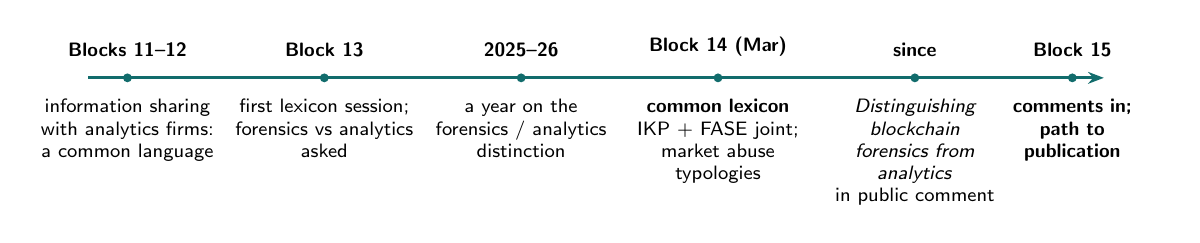
\begin{tikzpicture}[font=\scriptsize]
    \draw[line width=1pt,aml,-{Stealth[length=2mm]}] (0,0) -- (12.9,0);
    \foreach \x/\lab/\txt in {
      0.5/Blocks 11--12/{information sharing\\ with analytics firms:\\ a common language},
      3.0/Block 13/{first lexicon session;\\ forensics vs analytics\\ asked},
      5.5/2025--26/{a year on the\\ forensics / analytics\\ distinction},
      8.0/Block 14 (Mar)/{\textbf{common lexicon}\\ IKP + FASE joint;\\ market abuse typologies},
      10.5/since/{\emph{Distinguishing blockchain}\\ \emph{forensics from analytics}\\ in public comment},
      12.5/Block 15/{\textbf{comments in;}\\ \textbf{path to}\\ \textbf{publication}}}
      {\fill[aml] (\x,0) circle (1.6pt);
       \node[above=1.5mm,align=center,font=\scriptsize\bfseries] at (\x,0) {\lab};
       \node[below=1.5mm,align=center,text width=2.3cm] at (\x,0) {\txt};}
  \end{tikzpicture}
  \end{center}
  \par\vspace{2mm}
  \amllead{Two outcomes were asked for at Block 14: a \textbf{common language} (and possibly a shared database) for what practitioners see, and \textbf{getting the terminology right} between what is analytic understanding of chain data and what can stand as forensic evidence in court. Both are served by one lexicon.}
  \takeaway{The problem was never a lack of definitions. It is the cacophony of them.}
\end{frame}

% ================================================================ 29 forensics vs analytics
\begin{frame}{Forensics versus Analytics --- Settling the Framing}
  \begin{center}\scriptsize
  \begin{tabular}{@{}p{2.9cm}p{5.3cm}p{5.5cm}@{}}\toprule
     & \textbf{Blockchain analytics} & \textbf{Blockchain forensics}\\ \midrule
    Question answered & What is probably happening, at scale, now? & What happened, in this case, provably?\\
    Nature of the output & Probabilistic: heuristics, clustering, risk scores, typology matches & Evidentiary: attribution, chain of custody, reproducible method, documented limits\\
    Standard it meets & Fitness for a compliance or surveillance decision & Admissibility: reliability of method, error rate, expert testimony precedents\\
    Who uses it & VASPs, surveillance vendors, supervisors, researchers & Investigators, prosecutors, courts, counsel, regulators in enforcement\\
    Data it rests on & On-chain plus off-chain (venue, news, social); most activity is still off-chain & The same, with provenance of every input recorded\\
    Failure mode & False positives at scale; proprietary and unexplained signals & Over-claiming certainty from a probabilistic tool\\ \bottomrule
  \end{tabular}
  \end{center}
  {\scriptsize\color{soft} Precedents for probabilistic methods in evidence already exist (DNA matching, facial recognition), including how error rates and disclosure duties were handled.}
  \takeaway{Analytics generates leads; forensics proves. A document that says which one a tool is doing, and when a result crosses from one to the other, is the deliverable.}
\end{frame}

% ================================================================ 30 lexicon in progress
\begin{frame}{The Common Lexicon --- Terms in Progress}
  \amllead{Block 14 started from market abuse, where the typologies are most crypto-specific and the data is richest; AML/CFT terms, where much is not unique to crypto, are mapped rather than redefined.}
  \begin{center}\scriptsize
  \begin{tabular}{@{}p{2.4cm}p{5.0cm}p{6.4cm}@{}}\toprule
    \textbf{Family} & \textbf{Terms in progress} & \textbf{Observed signal}\\ \midrule
    Market abuse & Insider trading; pump and dump, incl. cross-venue pumps; touting (social or news driven) & Pre-announcement accumulation on-chain (one survey: clear signals in 56\% of listings studied); 15-minute venue pumps; off-chain news as data\\
    Scams by construction & Hard-coded rug pull; honeypot; related sub-typologies & Contract code present at deployment that has no legitimate purpose; detectable at the moment of deployment\\
    Wash trading & A-to-A; multi-party; cross-symbol (prediction markets) & Non-economic trading in swap pools and order books; the term was built for central limit order books and has to be re-defined for pools\\
    AML / CFT & Sanctions exposure; laundering through non-economic trading; mixing & More binary than market abuse: touched the sanctioned actor or did not. Maps to FATF, FinCEN red-flag advisories and national rules rather than inventing terms\\ \bottomrule
  \end{tabular}
  \end{center}
  {\scriptsize\color{soft} ``One person's wash trading is another's launch strategy.'' Market-abuse lines are drawn by law and settled by courts; the lexicon records the typology and the signal, not the verdict.}
  \takeaway{Mapping first, defining second: what definitions exist (ISO TC 307 vocabulary, FATF, national rules), where they conflict, and only then where a new term is needed.}
\end{frame}

% ================================================================ 31 machine-readable
\begin{frame}{From Lexicon to Something Machines Can Use}
  \begin{center}
  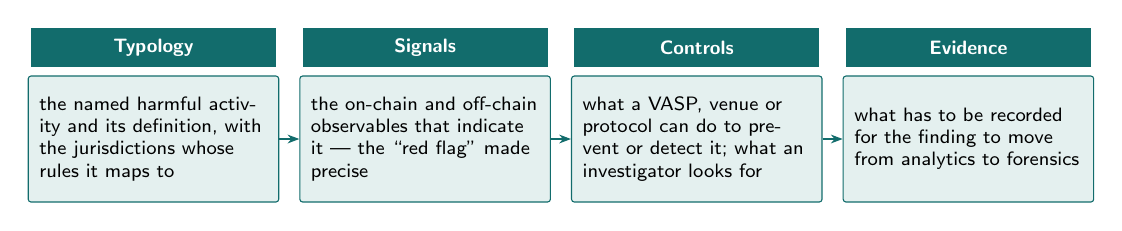
\begin{tikzpicture}[font=\scriptsize, box/.style={draw=aml,fill=amlbg,rounded corners=1pt,text width=2.9cm,align=left,inner sep=4pt,minimum height=1.6cm}, hd/.style={fill=aml,text=white,font=\scriptsize\bfseries,text width=2.9cm,align=center,inner sep=3pt,minimum height=5mm}]
    \foreach \i/\h/\t in {0/Typology/{the named harmful activity and its definition, with the jurisdictions whose rules it maps to},1/Signals/{the on-chain and off-chain observables that indicate it --- the ``red flag'' made precise},2/Controls/{what a VASP, venue or protocol can do to prevent or detect it; what an investigator looks for},3/Evidence/{what has to be recorded for the finding to move from analytics to forensics}}
      {\node[hd] (h\i) at (\i*3.45,0) {\h};
       \node[box,below=1mm of h\i] (b\i) {\t};}
    \foreach \i/\j in {0/1,1/2,2/3} \draw[-{Stealth[length=1.5mm]},aml] (b\i.east) -- (b\j.west);
  \end{tikzpicture}
  \end{center}
  \par\vspace{1.5mm}
  \begin{itemize}\small
    \item The shape of a \textbf{national vulnerability database}, for crypto harms: the Block 14 room pointed at the MITRE framework for crypto-specific exploitation as the nearest published precedent, and at BGIN's own cybersecurity information-sharing framework as the ``securitised'' sibling.
    \item \textbf{Formal over natural language where possible}: an ISO vocabulary standard takes three to four years; a standard that categorises a method or a mathematical object moves faster (the ISO 29128 experience).
    \item \textbf{Proprietary signals}: analytics firms may not disclose detection logic; the lexicon records typology and signal class, not vendor heuristics.
  \end{itemize}
  \takeaway{Two liaison organisations pushing the same taxonomy into ISO TC 307 is more impactful than one. BGIN is Category A; the mapping exercise is the lever.}
\end{frame}

% ================================================================ 32 privacy & proportionality
\begin{frame}{Privacy and Proportionality --- Inference and Its Limits}
  \amllead{A public ledger makes inference cheap. The question is not whether analytics is possible but what inferences are proportionate to the purpose, who may draw them, and what the subject can contest.}
  \begin{columns}[T]
    \begin{column}{0.48\textwidth}
      {\small\textbf{Three questions for every analytic}}
      \begin{itemize}\small
        \item \textbf{What} is inferred --- an address cluster, a counterparty, a person, a pattern of life?
        \item \textbf{By whom}, under what authority --- a VASP meeting its obligations, a vendor, a supervisor, law enforcement with process?
        \item \textbf{With what safeguards} --- retention, purpose limitation, error-rate disclosure, a route to contest a false positive?
      \end{itemize}
    \end{column}
    \begin{column}{0.48\textwidth}
      {\small\textbf{Where it meets this morning's session}}
      \begin{itemize}\small
        \item An unlinkable-by-design personhood credential and a sanctions-screening duty that presumes identifiability are on a collision course --- unclaimed elsewhere
        \item Privacy pools and ZK compliance proofs (Block 14 \emph{Accountable Wallet}): prove the property the rule requires, not the identity
        \item Cross-border information sharing carries the data-protection questions the Block 14 room flagged
      \end{itemize}
    \end{column}
  \end{columns}
  \takeaway{Proportionality is a lexicon term too: the document should say what level of inference each typology justifies, and what it does not.}
\end{frame}

% ================================================================ 33 guidance for three audiences
\begin{frame}{Guidance for VASPs, Investigators and Educators}
  \cpillar{aml}{0.31\textwidth}{VASPs}{Which typologies they are expected to detect; which signals are theirs to monitor and which are venue- or chain-level; when a hit is a lead and when it is evidence; what to record so that a later investigation can rely on it; how to buy or build capability without inheriting a vendor's undisclosed error rate.}\hfill
  \cpillar{aml}{0.31\textwidth}{Investigators}{How to assess the reliability of an analytics tool; what documentation moves a finding from probable to provable; the admissibility precedents for probabilistic methods; cross-border requests and the data-protection terms that go with them.}\hfill
  \cpillar{aml}{0.31\textwidth}{Educators}{The lexicon as a teaching instrument: one vocabulary for compliance teams, regulators and courts; typologies with worked public cases; the mutual education loop the Block 14 room described --- every conversation with a regulator teaches both sides.}
  \par\vspace{2.5mm}
  {\small Education was the one recommendation nobody argued with at Block 14: ``it was true five years ago, it is true today, it will be true forever, because things keep changing.''}
  \takeaway{Three audiences, one document, three reading paths through it.}
\end{frame}

% ================================================================ 34 discussion + next steps
\begin{frame}{Session 2-9 --- Discussion Items and the Path to Publication}
  \begin{columns}[T]
    \begin{column}{0.55\textwidth}
      \begin{enumerate}\small
        \item Which comments on the public-comment document change the \textbf{framing}, and which only the wording?
        \item Is the lexicon's scope \textbf{crypto-specific typologies} only, with general fraud and AML terms mapped to existing definitions --- or wider?
        \item What is the \textbf{minimum machine-readable record} for a typology entry, and who maintains it?
        \item Where does \textbf{proportionality} sit in the document --- a section, or a column on every entry?
        \item Which existing vocabularies does the mapping exercise \textbf{take as given} (ISO TC 307, FATF, national rules), and what is the process when they conflict?
      \end{enumerate}
    \end{column}
    \begin{column}{0.42\textwidth}
      {\small\textbf{Next steps toward publication}}
      \begin{itemize}\small
        \item Resolve comments; record each disposition
        \item Settle the forensics / analytics framing as the document's first section
        \item Lexicon v1: market abuse and scams-by-construction first; AML/CFT mapped
        \item Owners and date for the next iteration; the ISO TC 307 liaison route for the vocabulary
      \end{itemize}
    \end{column}
  \end{columns}
  \takeaway{Publish the framing document; keep the lexicon living, versioned and machine-readable.}
\end{frame}

% ================================================================ 35 what IKP leaves with
\begin{frame}{What IKP Leaves Block 15 With}
  \begin{center}\small
  \begin{tabular}{@{}p{3.2cm}p{5.6cm}p{4.9cm}@{}}\toprule
    \textbf{Session} & \textbf{Leaves with} & \textbf{Next stop}\\ \midrule
    1-4 / 1-7 PQC Migration & Committee seated; metric register v1; scheme-scope rulings and decision 0001 on record; open questions owned & W3 testbed (Nov); SSR workshop, 13 Dec (rubric v1, ``PQC-ready chain'', call text)\\
    2-6 PEA, ZKP \& PoP & Room comments into the personhood paper; the five distinctions and the unclaimed gaps confirmed as its structure; contributor list & Paper released for public comment; ISO TC 307 Technical Report path\\
    2-9 AML, Forensics \& Analytics & Comment dispositions; forensics / analytics framing settled; lexicon v1 scope and record shape & Publication of the framing document; lexicon maintained with FASE; ISO TC 307 liaison on vocabulary\\ \bottomrule
  \end{tabular}
  \end{center}
  \par\vspace{1mm}
  {\small Also carried: the Offline Key Management and Security AI Agent joint sessions (Cyber-chaired) take the same separation and at-rest principles into their guidance drafts.}
  \takeaway{Three public drafts went in; three records come out. Everything else is Discourse and pull requests between now and the next Block.}
\end{frame}

% ================================================================ 36 engage
\begin{frame}{How to Engage}
  \begin{columns}[T]
    \begin{column}{0.5\textwidth}
      \begin{itemize}\small
        \item \textbf{PQC}: nominate for the evaluation committee or a technical-advisor seat via the repository's issue template; comment on the metric register by pull request; the \emph{Post-Quantum Crypto Agility Competition} category on the BGIN Discourse.
        \item \textbf{Personhood}: read the Block 14 reports; add research questions to the ZKP / biometric authentication pathway thread; join the open IKP meetings; comment on the paper when it is released.
        \item \textbf{Forensics \& analytics}: comment on \emph{Distinguishing blockchain forensics from analytics}; bring a typology, a signal, or a case to the lexicon.
        \item \textbf{Everything}: the IKP and FASE categories on bgin.discourse.group. No salutations needed; the post carries the ask and the link.
      \end{itemize}
    \end{column}
    \begin{column}{0.47\textwidth}
      \begin{center}\tiny
        \begin{tabular}{@{}>{\centering\arraybackslash}p{2.2cm}@{\hspace{2mm}}>{\centering\arraybackslash}p{2.2cm}@{\hspace{2mm}}>{\centering\arraybackslash}p{2.2cm}@{}}
          \qrcode[height=1.5cm]{https://bgin-global.org/events/20261015-block15} &
          \qrcode[height=1.5cm]{https://github.com/bgin-global/pqc-agility-competition} &
          \qrcode[height=1.5cm]{https://bgin.discourse.group} \\[0.5mm]
          \textbf{Block 15 programme} & \textbf{Competition repository} & \textbf{BGIN Discourse} \\
          bgin-global.org/events/ 20261015-block15 & github.com/bgin-global/ pqc-agility-competition & bgin.discourse.group
        \end{tabular}
        \par\vspace{2mm}
        \begin{tabular}{@{}>{\centering\arraybackslash}p{2.2cm}@{\hspace{2mm}}>{\centering\arraybackslash}p{2.2cm}@{\hspace{2mm}}>{\centering\arraybackslash}p{2.2cm}@{}}
          \qrcode[height=1.5cm]{https://bgin-global.org/events/20261015-block15/sessions/1-4} &
          \qrcode[height=1.5cm]{https://bgin-global.org/events/20261015-block15/sessions/2-6} &
          \qrcode[height=1.5cm]{https://bgin-global.org/events/20261015-block15/sessions/2-9} \\[0.5mm]
          \textbf{1-4 / 1-7 PQC} & \textbf{2-6 PEA \& PoP} & \textbf{2-9 Forensics} \\
          \ldots/sessions/1-4 & \ldots/sessions/2-6 & \ldots/sessions/2-9
        \end{tabular}
      \end{center}
    \end{column}
  \end{columns}
  \takeaway{Discussion on Discourse; the documents and the repository are the record. Hybrid: remote participation details follow registration.}
\end{frame}

% ================================================================ 37 CLOSE
{\setbeamertemplate{footline}{}
\begin{frame}[plain]
  \begin{tikzpicture}[remember picture,overlay]
    \fill[bar] (current page.north west) rectangle (current page.south east);
    \node[anchor=south,text=white,font=\Large\bfseries,text width=13.5cm,align=center,execute at begin node=\nohyph] at ([yshift=6mm]current page.center){What a proof proves, and who is allowed to know.};
    \node[anchor=north,text=white,font=\small,text width=13.5cm,align=center,execute at begin node=\nohyph] at ([yshift=3mm]current page.center){Keys that outlive the primitive. Personhood without identity. Inference with limits. Written as criteria, taxonomy and lexicon --- not as a date, a provider, or a verdict.};
    \node[anchor=north,text=soft,font=\small,text width=13.5cm,align=center,execute at begin node=\nohyph] at ([yshift=-9mm]current page.center){BGIN IKP Working Group \textperiodcentered{} Mitchell Travers, Co-Chair \textperiodcentered{} bgin-global.org \textperiodcentered{} bgin.discourse.group};
    \node[anchor=south east,inner sep=0] at ([xshift=-7mm,yshift=5mm]current page.south east){
\includegraphics[height=1.4cm]{bgin_logo.png}};
  \end{tikzpicture}
\end{frame}}

\end{document}
